%---------------------%
%     Use of Scrum     %
%-------------------- %
\subsection{Use of Scrum}
\begin{frame}{Development Method}
  What is Scrum?
  \begin{itemize}
  \item Framework used to address complex adaptive problems
    \begin{itemize}
    \item Ensures products of highest possible value
    \end{itemize}
  \end{itemize}

	\begin{figure}
		\includegraphics[width=1\textwidth]{slides/agile-glossary.png}
	%	\caption{http://www.scrumhint.com/wp-content/uploads/2013/05/agile-glossary.png}
	\end{figure}
\end{frame}

\begin{frame}{Multi-Project Scrum usage}
  \begin{columns}
  		\begin{column}{0.5\textwidth}
  			Decision based on:
  			\begin{itemize}
      		\item Best-known methodology
      		\item Sprint length
        		\begin{itemize}
        		\item Fits study project well
        		\end{itemize}
      		\item Supported by tools
      		\item Recommended by Semester Coordinator
        \end{itemize}
  		\end{column}
  		
  		\pause
  		
  		\begin{column}{0.5\textwidth}
        Roles utilized:	
  	    \begin{itemize}
      	  \item Scrum Roles
        	  \begin{itemize}
        	    \item Scrum Master
        	  \end{itemize}
      		\item Ad-hoc Scrum Roles
        		\begin{itemize}
  	      		\item Client Contact
  	      		\item Sprint End Specialist
        		\end{itemize}
      	\end{itemize}
      	\pause
  	    \linespace
  			Worked only to a limited degree:
  			\begin{itemize}
  				\item Missing essential parts
    				\begin{itemize}
    				\item Product Owner
    				\item Scrum Master vs. Coordinator?
    				\end{itemize}
  			\end{itemize}
  		\end{column}
  \end{columns}
\end{frame}

\begin{frame}{Multi-Project Scrum usage}
  \begin{block}{Official Scrum Guide says:}
  \textit{''Scrum’s roles, artifacts, events, and rules are immutable and although implementing only parts of Scrum is possible, the result is not Scrum. 
  Scrum exists only in its entirety and functions well as a container for other techniques, methodologies, and practices.''}
  \end{block}
\end{frame}

\begin{frame}{Group Scrum usage}
	Intentions to form a Scrum of Scrums, to:
	\begin{itemize}
		\item Synchronize progress with multi-project Scrum
	\end{itemize}
	\begin{center}
	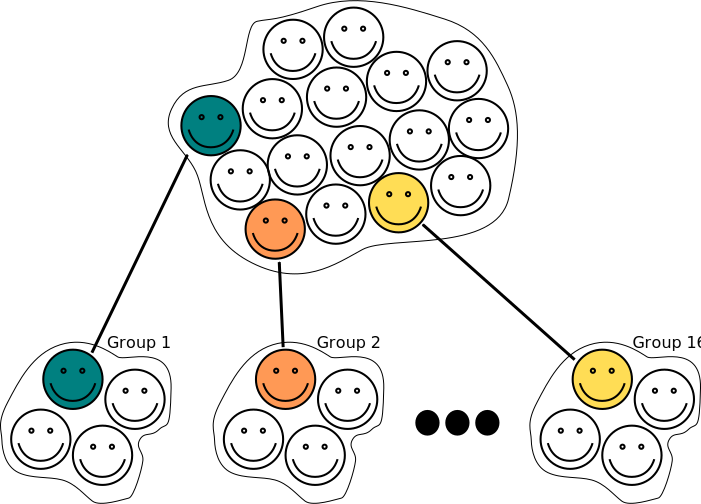
\includegraphics[width=0.6\textwidth]{pres/scrumofscrums}
	\end{center}
\end{frame}

\begin{frame}{Group Scrum usage}
  \begin{columns}
    \begin{column}{0.5\textwidth}
      Did not work as expected:
      \begin{itemize}
      	\item Failed to sustain Scrum Events
      			\begin{itemize}
      			\item Sprint Planning
      			\item Daily Scrum
       				\begin{itemize}
         				\item Scrum Board vs. Redmine
         				\item Shared group room
       				\end{itemize}
      			\item Sprint Review
      			\end{itemize}
        \item Did not utilize Scrum Roles
          \begin{itemize}
            \item Product Owner
            \item Scrum Master
          \end{itemize}
        \pause
        \item Scrum Retrospective
      \end{itemize}
    \end{column}
    
    \begin{column}{0.5\textwidth}
		\includegraphics[width=0.6\textheight]{slides/scrumboard}
		\\
		\linespace
		\includegraphics[width=0.6\textheight]{slides/redmine}
    \end{column}
  \end{columns}
\end{frame}

%--------------------------------------------------
%     OOD
%--------------------------------------------------
\subsection{System Design}
\begin{frame}{Developments}
	\begin{itemize}
		\item<1> Taking over an existing project
  		\begin{itemize}
    		\item Refactoring vs. Rewriting
  		\end{itemize}
		\item<2> Ad-hoc design
  		\begin{itemize}
  		\item Case: View Holder pattern, Android best-practice
  		\end{itemize}
		\begin{center}
		\includegraphics<1>[width=0.8\textheight]{slides/swengineer}
		\end{center}
	\end{itemize}
\end{frame}

\begin{frame}{Introducing Design Patterns}
  \begin{itemize}
  \item<1> Identify possible patterns to use
  \item<2> Suggestion: Observer Pattern
  \end{itemize}
  
  \includegraphics<2>[width=1\textwidth]{slides/observer.png}
\end{frame}



